\lecture{18}{9. April 2025}{Development of Microstructure and Alteration of Mechanical Properties}

\subsection{The kinetics of phase transformations}
Under a phase transformation, normally at least one new phase is formed that has different physical or chemical characteristics and/or a different structure than the parent phase. Also, most phase transformations are not instantaneous. Rather they begin by the formation of numerous small particles of the new phase(s), which increase in size until the transformation has reached completion. On this basis, the progress of a phase transformation may be broken down into two distinct stages: nucleation and growth. 

During nucleation small particles (nuclei) appear. These often consist of only a few hundred atoms and are capable of growing. During the growth stage, these nuclei increase in size, which result in the dissappearance of some or all of the parent phase. 

\subsubsection{Nucleation}
One typically distinguishes between two main types of nucleation: \textit{homogeneous} and \textit{heterogeneous}. The distinction between them is made according to the site at which nucleation occurs. For the homogeneous type, nuclei of the new phase form uniformally throughout the parent phase, whereas for the heterogeneous type, nuclei form preferentially at structural inhomogeneities, such as container surfaces, insoluble impurities, grain boundaries, and dislocations.

\paragraph{Homogeneous nucleation} To understand nucleation one also needs to know about the \textit{Gibbs free energy}, $G$. In brief, free energy is a function of other thermodynamic parameters, of which one is the internal energy of the system (i.e. Enthalpy $H$) and another is the entropy of the system. Relative to phase transformations, an important thermodynamic parameter is especially the change in free value $\Delta G$; a transformation occurs only spontaneously when $\Delta G$ has a negative value.

If we consider the solidification of a pure material, assuming that nuclei of the solid phase form in the interior of the liquid as atoms cluster together so as to form a packing arrangement similar to that found in the solid phase.

It is assumed that each nucleus is spherical and has a radius $r$. There are two contributions to the total free energy change that accompany a solidification transformation. The first is the free energy difference between the solid and liquid phases, or the volume free energy, $\Delta G_V$. Its value is negative if the temperature is below the equilibrium solidification temperature, and the magnitude of its contribution is the product of $\Delta G_v$ and the volume of the spherical nucleus. The second energy contribution results from the transformation of the solid-liquid phase boundary during the solidification transformation. Associated with this boundary is a surface free energy, $\gamma$, which is positive; furthermore, the magnitude of this contribution is the magnitude of this and the surface area of the nucleus. Finally the total free energy change is equal to the sum of these two contributions:
\[ 
\Delta G = \frac{4}{3}\pi r^3 \Delta G_v + 4 \pi r^2 \gamma
.\]
From this it can be seen that this sum (the free energy) actually first increases, before passing through a maximum and decreasing. In a physical sense this means that as a solid particle begins to form its free energy first increases. If the cluster reaches a size corresponding to the critical radius $r^{*}$ then growth will continue with an accompagniement of a decrease in free energy. However, a cluster of radius less than the critical value will shrink and redissolve. A subcritical particle is called an \textit{embryo} and a particle of radius greater than critical is termed a \textit{nucleus}. 

A critical free energy, $\Delta G^{*}$, occurs at the critical radius. This corresponds to the \textit{activation free energy}, which is the free energy required for the formation of a stable nucleus. We can find the critical radius and activation free energy as:
\begin{align*}
  r^{*} &= - \frac{2\gamma}{\Delta G_v} \\
  \Delta G^{*} &= \frac{16\pi \gamma^3}{3 \left( \Delta G_v \right)^2}
.\end{align*}
This volume free energy change $\Delta G_v$ is the driving force for the solidification transformation, and its magnitude is a function of temperature. At the equilibrium solidification temperature $T_m$, the value of $\Delta G_v$ is zero, and with decreasing temperature its value becomes increasingly negative. It can be shown that $\Delta G_v$ is a function of temperature as:
\[ 
\Delta G_v = \frac{\Delta H_f \left( T_m - T \right) }{T_m}
\]
where $\Delta H_f$ is the latent heat of fusion, and $T_m$ and the temperature $T$ are in Kelvin. One can also express the critical radius and activation free energy in terms of this as:
\begin{align*}
  r^{*} &= \left( - \frac{2\gamma T_m}{\Delta H_f} \right) \left( \frac{1}{T_m - T} \right)  \\
  \Delta G^{*} &= \left( \frac{16 \pi \gamma^3 T_m^2}{3 \Delta H_f^2} \right) \frac{1}{\left( T_m - T \right)^2}
.\end{align*}
From these two equations it can be seen that both the critical radius and the activation free energy decrease as the temperature decreases. 

Furthermore, the number of stable nuclei $n^{*}$ (having radii greater than $r^{*}$) is a function of temperature as
\[ 
n^{*} = K_1 e^{- \frac{\Delta G^{*}}{kT}}
\]
where the constant $K_1$ is related to the total number of nuclei of the solid phase.

Another important temperature-dependent step is involved in and also influences nucleation: the clustering of atoms by short-range diffusion during the formation of nuclei. This diffusion effect is related to the frequency at which atoms from the liquid attach themselves to the solid nucleus $v_d$. The dependence of $v_d$ on temperature is the same as for the diffusion coefficient, namely:
\[ 
v_d = K_2 e^{-\frac{Q_d}{kT}}
\]
where $Q_d$ is a temperature-independent parameter -- the activation energy for diffusion -- and $K_2$ is a temperature-independent constant. Therefore a decrease in temperature results in a reduction in $v_d$. 

Another important parameter is the nucleation rate $\dot{N}$ (which has units of nuclei per unit volume per second). This rate is simply proportional to the product of $n^{*}$ and $v_d$ as
\[ 
\dot{N} = K_3 n^{*} v_d = K_1 K_2 K_3 e^{- \frac{\Delta G^{*}}{kT}} e^{- \frac{Q_d}{kT}}
.\]
Here $K_3$ is the number of atoms on a nucleus surface.

\paragraph{Heterogeneous nucleation} It is often easier for nucleation to occur at surfaces and interfaces than at other sites. In order to understand this, we consider the nucleation, on a flat surface, of a solid particle from a liquid phase. It is assumes that both the liquid and solid phases ``wet'' this flat surface -- that is, they both spread out and cover the surface. Taking a surface tension force balance in the plane of the flat surface leads to the following expression:
\[ 
\gamma_{IL} = \gamma_{SI} + \gamma_{SL} \cos \theta
.\]
One can derive the equations for $r^{*}$ and $\Delta G^{*}$ to be:
\begin{align*}
  r^{*} &= - \frac{2\gamma_{SL}}{\Delta G_v} \\
  \Delta G^{*} &= \left( \frac{16 \pi \gamma^3_{SL}}{3 \Delta G_v^2} \right) S(\theta)
.\end{align*}
The $S(\theta)$ term is a function only of $\theta$ (i.e. the shape of the nucleus), which has a numerical value between 0 and 1. 


\subsubsection{Growth}
The growth step in a phase transformation begins once an embryo has exceeded the critical size $r^{*}$ and becomes a stable nucleus. Particle growth occurs by long-range atomic diffusino, which normally involves several steps -- for example, diffusion through the parent phase, across a phase boundary and then into the nucleus. Consequently, the growth rate $\dot{G}$ is determined by the rate of diffusion:
\[ 
\dot{G} = C e^{- \frac{Q}{kT}}
.\]
Where $Q$ (activation energy) and $C$ (constant) are independent of temperature. 


\subsubsection{Kinetic considerations of Solid-State Transformations}
Within many kinetic investigations, the fraction of reaction that has occured is measured as a function of time while the temperature is maintained constant. Data are plotted as the fraction of transformed material versus the logarithm of time. For most solid-state transformations the fraction of transformation $y$ is a function of time $t$ as:
\[ 
y = 1 - e^{- kt^{n}}
.\]
where $k$ and $n$ are time independent constants for the particular reaction. This is sometimes called the \textit{Avrami equation}. By convention the rate of transformation if taken as the reciprocal of time required for the transformation to proceed halfway to completion, $t_{\num{0,5} }$ or:
\[ 
\mathrm{rate} = \frac{1}{t_{\num{0,5} }}
.\]

\subsection{Isothermal transformation diagrams}

\paragraph{Pearlite}
Consider the iron-iron carbide eutectoid reaction:
\[ 
\gamma \left( \qty{0,76}{wt \% C} \right) \alpha \left( \qty{0,022}{wt\% C} \right) + \mathrm{Fe}_3 \mathrm{C}\left( \qty{6,70}{wt\% C}  \right)
.\]
Upon cooling, austenite, having an intermediate carbon concentration, transforms into a ferrite phase, which has a much lower carbon content, and also cementite, which has a much higher carbon concentration. The temperatue dependence of this is shown in \textbf{\autoref{fig:e19_1}}.
\begin{figure} [ht]
  \centering
  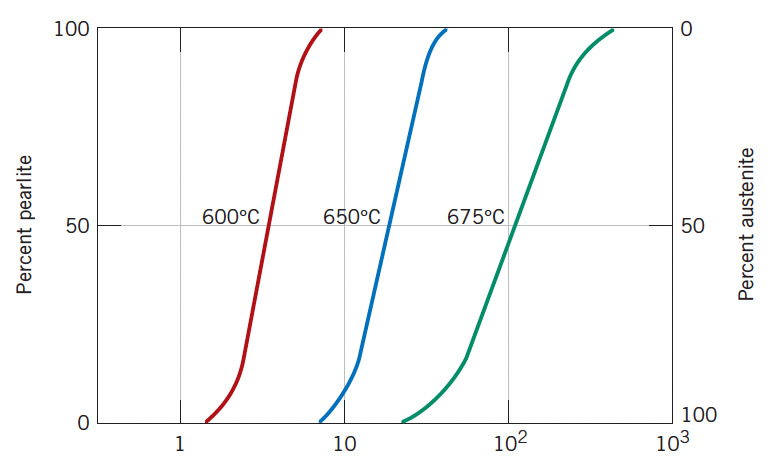
\includegraphics[width=0.5\linewidth]{./figures/e19_1.png}
  \caption{Temperature dependence of the austenite to pearlite transformation}
  \label{fig:e19_1}
\end{figure}

A more convenient way of representing both the time and temperature depdendence of this transformation is shown in \textbf{\autoref{fig:e19_2}}.
\begin{figure} [ht]
  \centering
  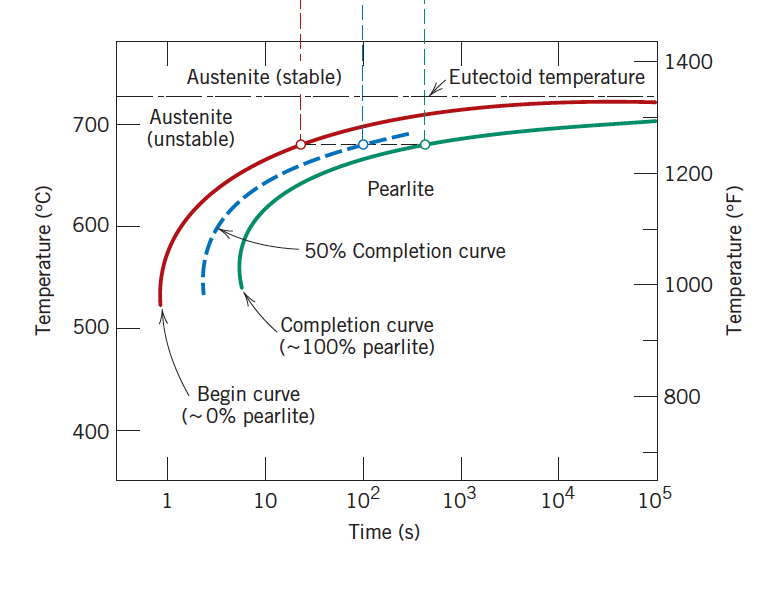
\includegraphics[width=0.5\linewidth]{./figures/e19_2.png}
  \caption{Temperature dependence of the transformation} 
  \label{fig:e19_2}
\end{figure}
Here, the vertical and horizontal axes, are respectively, temperature and the logarithm of time. Two solid curves are plotted; one represents the time required at each temperature for the initiation or start of the transformation and the other is for the transformation conclusion. The dashed curve corresponds to 50\% of transformation completion. One must note that this is only valid for the mixture at eutectiod composition.


